\documentclass{article}
\usepackage[UTF8]{ctex}
\usepackage[T1]{fontenc}
\usepackage[utf8]{inputenc}
\usepackage{latexsym}
\usepackage{amsmath}
\usepackage{amsthm}
\usepackage{amssymb}
\usepackage{clrscode3e}
\usepackage{xcolor}
\usepackage{tikz}
\usepackage{tkz-berge}
\usepackage[position=top]{subfig}
\usetikzlibrary{arrows, petri, topaths}

\title{Homework 10}
\author{PB17000297 罗晏宸}
\date{December 26 2019}

\begin{document}

\maketitle

\section{Exercise 34.5-1}
\textbf{子图同构问题}取两个无向图 $G_1$ 和 $G_2$, 要回答 $G_1$ 是否与 $G_2$ 的一个子图同构这一问题。证明:子图同构问题是 NP 完全的。

\paragraph{解}
首先证明子图同构问题是属于 NP 的,在多项式的时间内是可以对子图同构问题的答案给出验证,即验证给定的 $G_2$ 的子图是否与 $G_1$ 同构。\par
下面证明子图同构问题是 NP 难度的,如果能够在多项式的时间内解决子图同构问题,取 $G_1$ 是一个顶点数为 $k$ 的完全图,则能够在多项式的时间内解决\textbf{团问题}:在 $G_2$ 中是否存在一个给定规模为 $k$ 的团。\par
综上,子图同构问题是 NP 完全的。

\section{Exercise 34.5-6}
证明:哈密顿路径问题是 NP 完全的。

\paragraph{解}
首先一条从$u$ 到 $v$ 的 Hamilton 路径即哈密顿路径问题的证书,这说明哈密顿路径问题是属于 NP 的。\par
对于顶集覆盖问题中的输入$G$与$k$,下面通过证明 $\text{VERTEX-COVER} \\ \leq_\text{P} \text{HAM-PATH}$来证明哈密顿路径问题是 NP 难度的。首先 $\forall v \in V(G)$,将$v$分为 $2d(v)$ 个顶点:$v(1,1), v(1, 2) , \cdots , v(2, d(v))$,再添加 $k$个新顶点:$u_0 = a_0, a_1, a_2, \cdots , a_k = v_0$,以上顶点构成$V(G')$。在上述顶集中连边:$\forall v \in V(G)$,连边$v(1,i)v(2,i), \ i = 1, \cdots , d(v)$,$v(2,i)v(1,i + 1), \ i = 1, \cdots , d(v) - 1$,$v(1,1)a_i, \ i = 1, \cdots , k - 1$,$v(2,d(v))a_i, \ i = 1, \cdots , k$;$\forall uv \in E(G)$,设$uv$是$G$中与$u$相关联的第$i$条边、与$v$相关联的第$j$条边,则连边$u(1,i)v(1,j)$与$u(2,i)v(2,j)$。以上边构成$E(G')$。\par
上述$G'$的构造是多项式时间内可以完成的。下面证明$G$中有$k$个顶组成的顶覆盖当且仅当$G'$中有哈密顿路径$P(u_0, v_0)$。\par
事实上,若$G$中有一个顶覆盖$C = {v_1, v_2, \cdots, v_k}$,在$G'$中,从$u_0$出发,通过一条边到达$v_1(1,1)$,继而沿路径$v_1(1,1)v_1(2,1)v_1(1,2)v_1(2,2)v_1(1,3) \\ v_1(2,3)\cdots v_1(2,d(v_1))$,再从$v_1(2,d(v_1))$到达$a_1$;再从$a_1$出发,通过一条边到达$v_2(1,1)$,继而沿路径$v_2(1,1)v_2(2,1)v_2(1,2)v_2(2,2)v_2(1,3)v_2(2,3) \cdots \\ v_2(2,d(v_2))$,再从$v_2(2,d(v_2))$到达$a_2$;依次前进$k$轮,最终从$v_k(2,d(v_k))$出发,通过一条边到达$a_k = v_0$,得到了$G'$中的路径$P_1(u_0, v_0)$。若$P_1(u_0, v_0)$不是哈密顿路径,任取$v \notin {v_1, v_2, \cdots, v_k}$,且$e = uv \in E(G)$,设$e = uv$是$G$中与$u$相关联的第$i$条边、与$v$相关联的第$j$条边,则$u \in {v_1, v_2, \cdots, v_k}$,用路径$u(1, i)v(1, j)v(2, j)u(2, i)$代替$P_1$中的$u(1,i)u(2,i)$,得到$P_2$,直到扩张得到哈密顿路径$P(u_0, v_0)$。\par
若$P(u_0, v_0)$是$G'$中的一条哈密顿路径,仅当$v(1,1)$与$v(2, d(v))$在$P(u_0, v_0)$上均与${a_0, a_1, \cdots, a_k}$中的顶点相邻时,$v$加入顶点覆盖$S$,故$|S| = k$。\par
因此,哈密顿路径问题是 NP 难度的。综上,哈密顿路径问题是 NP 完全的。

\section{Exercise 35.2-4}
在\textbf{瓶颈旅行商问题}中,目标是找出这样一条哈密顿回路,使得回路中代价最大的边的代价相对于其他回路来说最小。假设代价函数满足三角不等式,证明:这个问题存在一个近似比为 3 的多项式时间近似算法。

\paragraph{解}
对于图的最小生成树,从某一顶点开始,在图中依次取点完成一个哈密顿回路,每次经过边的端点在最小生成树上的距离不超过3,设$C$是求出最小生成树的代价,则前述过程的代价最多为$3C$。设最优解的代价为$C*$,对于同一个图,设求出瓶颈哈密顿路径的代价为$C'$,显然从一条瓶颈哈密顿路径可以通过依次删除按代价排序的边得到最小生成树,而$C* < C‘$,因此有$C* < C' < 3C$,即前述算法是3近似的。

\section{Problem 35-6 Approximating a maximum spanning tree}
设 $G = (V, E)$ 是一个无向图,其中的每条边 $(u, v) \in E$ 具有不同的权值 $w(u,v)$。对每个顶点 $v \in V$,设 $\max{(v)} = \displaystyle \arg{\max_{(u,v) \in E}{\{ w(u, v) \}}}$ 是与顶点 $v$ 相关联的最大权值边。设 $S_G = \{ \max{(v)} : v \in V\} $ 表示与各个顶点相关联的最大权值边的集合,$T_G$ 表示图 $G$ 的最大权值生成树。对任意的边集 $E' \subseteq E$,定义 $w(E') = \displaystyle \sum_{(u,v) \in E'}{w(u,v)}$。
\subparagraph{a} 给出一个至少包含 4 个顶点的图,使其满足 $S_G = T_G$。
\subparagraph{b} 给出一个至少包含 4 个顶点的图,使其满足 $S_G \neq T_G$。
\subparagraph{c} 证明:对任意的图 $G$,$S_G \subseteq T_G$。
\subparagraph{d} 证明:对任意的图 $G$,$w(T_G) \geq w(S_G) / 2$。
\subparagraph{e} 给出一个 $O(V + E)$ 时间算法,用于计算 2 近似的最大生成树。


\paragraph{解}
\subparagraph{a}
\begin{figure}[H]
    \centering
    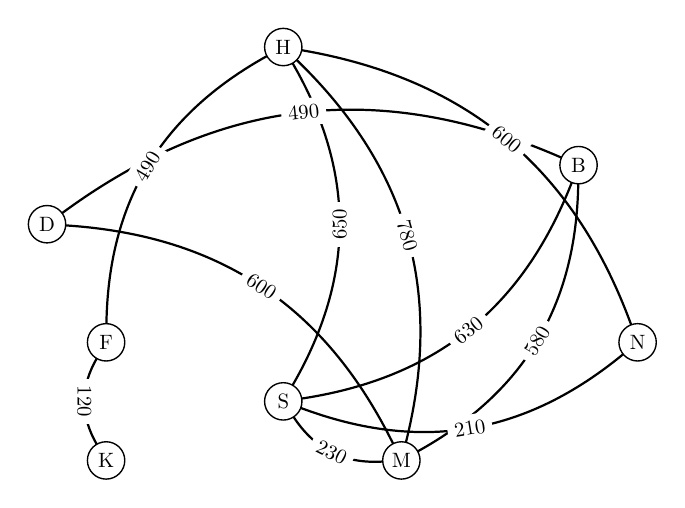
\begin{tikzpicture}[scale=0.75, transform shape]
      \Vertex[x=0, y=0] {K}
      \Vertex[x=0, y=2] {F}
      \Vertex[x=-1, y=4]{D}
      \Vertex[x=3, y=7] {H}
      \Vertex[x=8, y=5] {B}
      \Vertex[x=9, y=2] {N}
      \Vertex[x=5, y=0] {M}
      \Vertex[x=3, y=1] {S}
      \tikzstyle{LabelStyle} = [fill = white, sloped]
      \tikzstyle{EdgeStyle} = [bend left]
      \Edge[label=$120$](K)(F)
      \Edge[label=$650$](H)(S)
      \Edge[label=$780$](H)(M)
      \Edge[label=$490$](D)(B)
      \Edge[label=$600$](D)(M)
      \Edge[label=$580$](B)(M)
      \Edge[label=$600$](H)(N)
      \Edge[label=$490$](F)(H)
      \tikzstyle{EdgeStyle}=[bend right]
      \Edge[label=$630$](S)(B)
      \Edge[label=$210$](S)(N)
      \Edge[label=$230$](S)(M)
    \end{tikzpicture}
\end{figure}
\subparagraph{b}
\subparagraph{c}
\subparagraph{d}
\subparagraph{e}

\section{Exercise 34.4-7}
给出一种 2-SAT 问题的多项式解法
\paragraph{解}

\end{document}